\documentclass{article}


\usepackage{amsmath,amsfonts,amsthm,amssymb,amsopn,bm}
% \usepackage{fullpage}
\usepackage[margin=.9in]{geometry}
\usepackage{graphicx}
% \usepackage{fullpage}
% \usepackage[paper=letterpaper,margin=1in,includeheadfoot,footskip=0.25in,headsep=0.25in]{geometry}
\usepackage{url}
\usepackage[usenames,dvipsnames]{color}
% \usepackage[pdfborder={0 0 1},colorlinks=true,citecolor=black,plainpages=false]{hyperref}
\usepackage{fancyhdr}
\usepackage[ruled]{algorithm2e}
\usepackage{listings}
% \usepackage{multirow}
\newcommand{\field}[1]{\mathbb{#1}}
\newcommand{\1}{\mathbf{1}}
\newcommand{\E}{\mathbb{E}} % real domain
\renewcommand{\P}{\mathbb{P}} % real domain
\newcommand{\R}{\field{R}} % real domain
% \newcommand{\C}{\field{C}} % complex domain
\newcommand{\F}{\field{F}} % functional domain

\newcommand{\T}{^{\textrm T}} % transpose


\def\diag{\text{diag}}

%% operator in linear algebra, functional analysis
\newcommand{\inner}[2]{#1\cdot #2}
\newcommand{\norm}[1]{\left\|#1\right\|}
\newcommand{\twonorm}[1]{\|#1\|_2^2}
% operator in functios, maps such as M: domain1 --> domain 2
\newcommand{\Map}[1]{\mathcal{#1}}
\renewcommand{\theenumi}{\alph{enumi}} 

\newcommand{\Perp}{\perp \! \! \! \perp}

\newcommand\independent{\protect\mathpalette{\protect\independenT}{\perp}}
\def\independenT#1#2{\mathrel{\rlap{$#1#2$}\mkern2mu{#1#2}}}
\newcommand{\vct}[1]{\boldsymbol{#1}} % vector
\newcommand{\mat}[1]{\boldsymbol{#1}} % matrix
\newcommand{\cst}[1]{\mathsf{#1}} % constant
\newcommand{\ProbOpr}[1]{\mathbb{#1}}
\newcommand{\grade}[1]{\small\textcolor{magenta}{\emph{[#1 points]}} \normalsize}
\date{{}}

\setlength\parindent{0px}

\begin{document}
\title{Homework \#2}
\author{\normalsize{CSE 546: Machine Learning}\\
\normalsize{Michael Ross}}
\maketitle

\section{A Taste of Learning Theory}
1. \grade{2}
Let $X$ be a random feature vector in $\R^d$ and $Y$ be a random label in $\{1,\dots,K\}$ for some $K \in \mathbb{N}$ drawn from a joint distribution $P_{XY}$. 
A \emph{randomized classifier} $\delta(x)$ takes an $x\in \R^d$ as input and outputs an element $y \in \{1,\dots,K\}$ with probability $\alpha(x,y) := P(\delta(x) = y)$, where $\sum_{y=1}^K \alpha(x,y) = 1$ for all $x$.
For any classifier $\delta$ we define the \emph{risk} as
\begin{align*}
R(\delta) := \E_{XY,\delta}[ \1\{ \delta(X) \neq Y \}]
 % = \E_X[ \E_{Y|X}[ \1\{\delta(x) \neq Y \} | X=x ] ]
\end{align*}
where $\1(\mathcal{E})$ is the indicator function for the event $\mathcal{E}$ (the
function takes the value $1$ if $\mathcal{E}$ occurs and $0$ otherwise).
We say a classifier $\delta$ is \emph{deterministic} if $\alpha(x,y) \in \{0,1\}$ for all $x,y$.
A Bayes classifier is defined as $\delta_* \in \arg\inf_\delta R(\delta)$ where the infimum is taken over all randomized classifiers (note it may not be unique). 
For an arbitrary $P_{XY}$, characterize the set of all Bayes Classifiers (i.e., for a given $x$ what are permissible Bayes classifiers in terms of $\alpha(x,y)$).
Then propose a deterministic decision rule that is a Bayes classifier.\\

\textbf{Answer:}\\
$R(\delta) = \E_{XY,\delta}[ \1\{ \delta(X) \neq Y \}]$\\
$= \E_{XY}[ \E_{\delta}[\1\{ \delta(x) \neq y \} | X=x, Y=y]]$\\
$= \E_{XY}[ \alpha(X,Y)]$\\
$=\sum_{y=1}^K \int_0^\infty P_{XY} \alpha(x,y) dx $\\
$\leq \sum_{y=1}^K \int_0^\infty P_{XY} \text{ max} (\alpha(x,y)) dx $\\
$\leq \text{ max} (\alpha(x,y)) \sum_{y=1}^K \int_0^\infty P_{XY}  dx $\\

$\sum_{y=1}^K \int_0^\infty P_{XY}  dx = 1$ due to conservation of probability\\



2. \grade{8} 
For $i=1,\dots,n$ let $(x_i,y_i) \overset{i.i.d.}{\sim} P_{XY}$ where $y_i \in \{-1,1\}$ and $x_i$ lives in some set $\mathcal{X}$ ($x_i$ is not necessarily a vector). 
The $0/1$ loss, or \emph{risk}, for a deterministic classifier $f:\mathcal{X} \rightarrow \{ -1,1 \}$ is defined as:
\begin{align*}
R(f) = \mathbb E_{XY} [\1(f(X)\neq Y)]
\end{align*}
where $\1(\mathcal{E})$ is the indicator function for the event $\mathcal{E}$ (the
function takes the value $1$ if $\mathcal{E}$ occurs and $0$ otherwise).
The expectation is with respect to the underlying distribution $P_{XY}$ on $(X,Y)$.
Unfortunately, we don't know $P_{XY}$ exactly, but we do have our i.i.d. samples $\{(x_i,y_i)\}_{i=1}^n$ drawn from it.
Define the \emph{empirical risk} as 
\begin{align*}
\widehat R_n(f) = \frac{1}{n} \sum_{i=1}^n \mathbf{1}(f(x_i)\neq y_i) 
\end{align*}
which is just an empirical estimate of our loss.
Recall Hoeffding's inequality: if $Z_1,\dots,Z_m$ are i.i.d. random variables on the interval $[a,b]$ where $\E[Z_i] = \mu$ and $\widehat{\mu} = \frac{1}{m} \sum_{i=1}^m Z_i$, then 
\begin{align*}
\P\left( |\mu - \widehat{\mu}| \geq \epsilon \right) \leq 2 \exp\left(- \frac{2 m \epsilon^2}{(b-a)^2}\right).
\end{align*}

\begin{enumerate}
  \item Suppose a domain expert who has not seen your freshly drawn data $\{(x_i,y_i)\}_{i=1}^n$ gives you a classifying rule $\widetilde{f}:\mathcal{X} \rightarrow \{-1,1\}$. We wish to estimate the true risk $R(\widetilde{f})$ of this classifying rule using the empirical risk $\widehat{R}_n(\widetilde{f})$. Justify the use of Hoeffding's inequality, and use it to find a value of $A$ such that
  \begin{align*}
  \P( | \widehat{R}_n(\widetilde{f}) - R(\widetilde{f}) | \leq A ) \geq 1- \delta.
  \end{align*}
  
  \textbf{Answer:}\\
   Since $\widetilde{f}$ was not created based on our drawn data and our drawn data are i.i.d, Hoeffding's inequality holds.\\
   $\P( | \widehat{R}_n(\widetilde{f}) - R(\widetilde{f}) | \leq A ) \geq 1- 2 \exp\left(- \frac{2 n A^2}{(1-(-1))^2}\right)$\\
   Let $\delta=2 \exp\left(- \frac{n A^2}{2}\right)$\\
   $A=\sqrt{\frac{2}{n}\log(\delta/2)} $
  
  \item After seeing the confidence interval, the domain expert is not satisfied with her classifying rule $\widetilde{f}$. Because she understands the underlying process that generated the data, she proposes a finite set of alternative classifying rules $\mathcal{F} = \{ f_1,\dots,f_k \}$ that may fit the data better.
  The ``best in class'' function $f^*$ is:
  \[
  f^* = \arg\min_{f \in \mathcal{F}} R(f) \, . 
  \]
  Note that $R(f^*)$ is the best true loss we could hope to achieve using functions in $\mathcal{F}$.
  If we replace $\widetilde{f}$ with $f^*$ in part a., does the same confidence interval hold? Why or why not?
  \item Of course, determining $f^*$ would require exact knowledge of $R(f)$, which requires exact knowledge of $P_{XY}$, which we don't have. 
  As an alternative, you propose to use the \emph{empirical risk minimizer} (ERM):
  \begin{align*}
  \widehat f = \arg\min_{f\in\mathcal{F}} \widehat R_n(f).
  \end{align*}
  If we replace $\widetilde{f}$ with $\widehat{f}$ in part a., does the same confidence interval hold? Why or why not? 
  \item Come up with a \textbf{simple} example (i.e., give a $P_{XY},\mathcal{F}$) where for any number of observations $n$ we have $\widehat{R}_n(\widehat{f})=0$ and $R(\widehat{f})=1/2$ where $\widehat{f} = \arg\min_{f \in \mathcal{F}} \widehat{R}_n(f)$.  
  \item  Provide a confidence interval that simultaneously holds for the losses of all $f \in \mathcal{F}$, with probability of error $\delta$. In other words, provide a value $B$ so that:
\[
\P( \textrm{for all } f\in\mathcal{F}, \, |\widehat R_n(f) -  R(f)|
\leq B ) \geq 1- \delta
\]
Show your steps. (Hint: for events $\mathcal{E}_1, \mathcal{E}_2, \ldots, \mathcal{E}_k$, the ``union bound'' states that  $\P(\mathcal{E}_1 \textrm{ or } \mathcal{E}_2 \textrm{ or } \dots \text{ or } \mathcal{E}_k) = \P(\bigcup_{i=1}^k \mathcal{E}_i ) \leq \sum_{i=1}^k \P(\mathcal{E}_k)$.)

\textbf{Answer:}\\
$\P( \textrm{for all } f\in\mathcal{F}, \, |\widehat R_n(f) -  R(f)| \leq B ) \geq 1- \delta = $\\

\item Noting that $\widehat{f} \in \mathcal{F}$, provide a confidence interval for the loss of $\widehat f$ that holds with
  probability greater than $1-\delta$. In other words, we are seeking
  a bound on $|R(\widehat f)-\widehat R_n(\widehat f)|$ that holds with probability greater than $1-\delta$.

\item Provide a bound on how close your loss, using the ERM, is
  to the best possible loss (in the hypothesis space). 
  Specifically, provide a value $C$ so that the following holds with probability greater than $1-\delta$,
  \[
  R(\widehat f) - R(f^*) \leq C
  \]
  The quantity $R(\widehat f) - R(f^*)$ is often referred to as the \emph{excess risk}.

\item Fix an $f \in \mathcal{F}$ and suppose $R(f) > \epsilon$. 
Show that $\P( \widehat{R}_n(f) = 0 ) \leq (1-\epsilon)^n \leq e^{-n \epsilon}$.
Leverage this insight to show that with probability at least $1-\delta$ 
\begin{align*}
\widehat{R}_n(\widehat{f})=0 \quad \implies \quad  R(\widehat f) - R(f^*) \leq \frac{\log(|\mathcal{F}|/\delta)}{n}
\end{align*}
where $\widehat f = \arg\min_{f\in\mathcal{F}} \widehat R_n(f)$. 

\item \label{last_part} Let us understand how large a hypothesis class we can utilize,
  i.e. how large $|\mathcal{F}|$ can be? Suppose we know we will be provided with a training set of
  size $n$, and, before we look at our training data, we choose the
  a hypothesis class $\mathcal{F}$ as a function of the sample size $n$. As we get
  more data, we would expect that we can utilize a larger hypothesis
  class. Let us examine this more quantitatively. We can think of
  learning being possible if our regret tends to $0$ as $n$ becomes
  large (with a probability of error less than  $\delta$). Let us determine if learning is possible in each of the
  following cases. For the following cases, does the above suggest that we are able to learn, and if so, what is our excess risk as a function of $n$ in big-O notation?
\begin{enumerate}
\item $|\mathcal{F}|$ is a constant.\\
\item $|\mathcal{F}|=n^p$ for some constant $p$.\\
\item $|\mathcal{F}|=\exp(\sqrt{n})$.\\
\item $|\mathcal{F}|=\exp(10 n)$. \\
\end{enumerate}
\end{enumerate}
Your answers to part \ref{last_part} are one interpretation as to when and why learning
complex models is possible (from a statistical perspective). 
Of particular interest is when $\mathcal{F}$ is allowed to be infinite in which more advanced tools are necessary. 
To provide intuition we note that $n$ points in $d$-dimensions can be labeled by a hyperplane $w$ in at most $O(n^d)$ ways (i.e., $|\{ \text{sign}(\mathrm{X} w) : w \in \R^d \}| = O(n^d)$ for fixed $\mathrm{X} \in \R^{n \times d}$).
While more advanced tools (e.g., VC dimension, covering numbers, etc.) are necessary to formally prove the learning rates for infinite classes, thinking about this number of sign patterns and how this relates to $|\mathcal{F}|$ is instructive.




\section{Programming: Lasso}

Given $\lambda >0$ and data $(x_1,y_1),\dots,(x_n,y_n)$, the Lasso is the problem of solving
\begin{equation}\label{eq:lasso}
  \arg\min_{{w}\in \R^d, b \in \R} \sum_{i=1}^n { (x_i^T {w} + b - {y}_i)^2 }
    + \lambda \sum_{j=1}^d |{w}_j| 
\end{equation}
$\lambda$ is a regularization tuning parameter.
For the programming part of this homework, you are required to implement the
coordinate descent method of Algorithm~\ref{alg:cd} that can solve the Lasso problem.\\
You may use common computing packages (such as NumPy or SciPy), but do not use an existing Lasso solver (e.g., of Sci-Kit Learn).

\begin{algorithm}[t]
    \caption{Coordinate Descent Algorithm for Lasso}\label{alg:cd}
    \While{not converged}{
      $b \leftarrow \frac{1}{n}\sum_{i=1}^n \left({y}_i - \sum_{j=1}^d {w}_j {x}_{i,j}\right)$\\ 
      \For{$k \in \{1,2,\cdots d\}$} {
        $a_k\leftarrow 2 \sum_{i=1}^n {x}_{i,k}^2$ \\   
        $c_k\leftarrow 2 \sum_{i=1}^n {x}_{i,k} \left({y}_i -(b + \sum_{j\neq k} {w}_j {x}_{i,j} )\right)$ \\
        ${w}_k \leftarrow 
        \left\{
        \begin{array}{ll}
          (c_k+\lambda) / a_k & c_k < -\lambda\\
          0 & c_k\in [-\lambda, \lambda]\\
          (c_k-\lambda) / a_k & c_k > \lambda\\
        \end{array}  
        \right.
        $
      }
    }
\end{algorithm}

Before you get started, here are some hints that you may find helpful:
\begin{itemize}
  \item For loops can be slow whereas vector/matrix computation in Numpy is very optimized, exploit this as much as possible.
  \item As a sanity check, ensure the objective value is nonincreasing with each step. 
  \item It is up to you to decide on a suitable stopping condition.  A common criteria is to stop when no element of
      ${w}$ changes by more than some small $\delta$ during an iteration.  If you need your algorithm to run faster,
      an easy place to start is to loosen this condition.
  \item You will need to solve the Lasso on the same dataset for many values of $\lambda$.  This
      is called a regularization path.  One way to do this efficiently is to start at a large $\lambda$, and then for
      each consecutive solution, initialize the algorithm with the previous solution, decreasing $\lambda$ by a constant
      ratio until finished.
  \item The smallest value of $\lambda$ for which the solution $\widehat{w}$ is entirely zero is given by
      \[ \lambda_{max} = \max_{k=1,\dots,d} 2 \left|\sum_{i=1}^n {x}_{i,k} \left({y}_i - \left(\frac{1}{n} \sum_{j=1}^n y_j \right)\right)\right| \]
      This is helpful for choosing the first $\lambda$ in a regularization path. 
\end{itemize}

3. \grade{5}  We will first try out your solver with some synthetic data.
A benefit of the Lasso is that if we believe many features are irrelevant for predicting ${y}$, the Lasso can be used to enforce a sparse solution, effectively differentiating between the relevant and irrelevant features.
Suppose that ${x} \in \mathbb{R}^d, y \in \mathbb{R}, k < d$, and pairs of data $({x}_i, y_i)$ for $i=1,\dots,n$ are generated independently according to the model $y_i = w^T x_i + \epsilon_i$ where
\begin{align*}
w_j = \begin{cases} j/k & \text{if } j \in \{1,\dots,k\} \\
0 & \text{otherwise}
\end{cases}
\end{align*} 
where $\epsilon_i \sim \mathcal{N}(0, \sigma^2)$ is some Gaussian noise (in the model above $b=0$).  Note that since $k < d$, the features $k + 1$ through $d$ are unnecessary (and potentially even harmful) for predicting $y$.

With this model in mind, let $n = 500, d = 1000, k = 100,$ and $\sigma = 1$.  Generate some data by drawing each $x_i \sim \mathcal{N}(0, I)$ so that $x_i \in \R^d$ with $y_i$ generated as specified above.
  \begin{itemize}
    \item  With your synthetic data, solve multiple Lasso problems on a regularization path, starting at $\lambda_{max}$ where $0$ features are selected and
  decreasing $\lambda$ by a constant ratio (e.g., 1.5) until nearly all the features are chosen.  
  In plot 1, plot the number of non-zeros as a function of $\lambda$ on the x-axis (Tip: use \verb|plt.xscale('log')|).
  \item  For each value of $\lambda$ tried, record values for false discovery rate (FDR) (number of incorrect nonzeros in $\widehat{w}$/total number of nonzeros in $\widehat{w}$) and true positive rate (TPR)
  (number of correct nonzeros in $\widehat{w}$/k).
  In plot 2, plot these values with the x-axis as FDR, and the y-axis as TPR and note that in an ideal situation we would have an (FDR,TPR) pair in the upper left corner, but that can always trivially achieve $(0,0)$ and $(\tfrac{d-k}{d},1)$ 
\end{itemize}      
  Comment on the effect of $\lambda$ in these two plots.\\
  
  \textbf{Answer:}\\
  
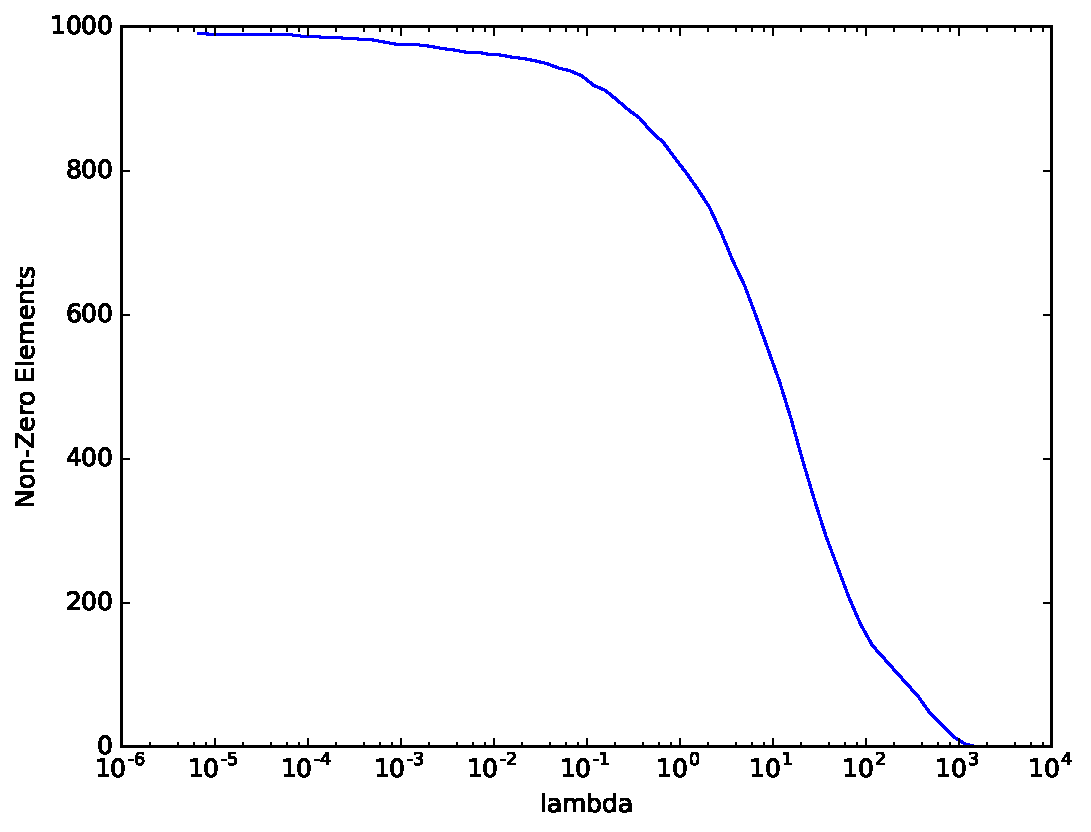
\includegraphics[width=4in]{NonzerovsLambda.pdf}\\
It's clear that at some point it becomes harder to add new non-zero features as lambda decreases. I find it interesting that at the point of the true number of non-zero features it appears that the curvature switches from positive to negative.

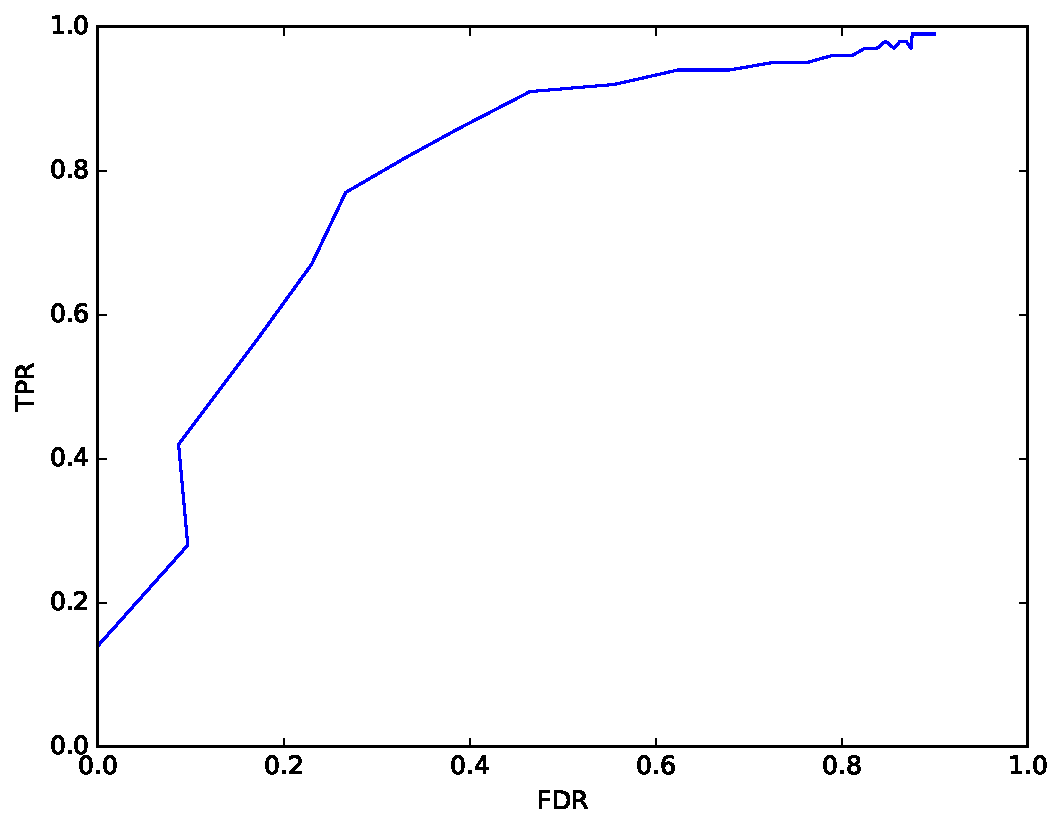
\includegraphics[width=4in]{FDRvsTPR.pdf}\\
The fact that as you increase from a small number of features the number of true detection rate increases quickly while the false discovery rate doesn't increase as much makes sense because the true values are easy to find in this regime. Then as you pass some point the TPR gets stuck and you add continue growing the FDR because most of the true non-zeros have already been found.\\

\textbf{Code:}
\begin{lstlisting}[language=Python]
import numpy as np
import matplotlib.pyplot as plt
import random
import time

n=500
d=1000
k=100
sigma=1

def generateSynth(n, d, k, sigma):
    x = sigma*np.random.randn(d, n)
    j = np.array(range(1, k+1))
    w = np.concatenate((j/k, np.zeros(d-k)))
    y = np.dot(w, x)+np.random.randn(n)
    return x, y, w

def coordDescent(x, y, lamb, delta, w0):
    d = x.T[0].size
    n=x[0].size

    a = np.zeros(d)
    c = np.zeros(d)
    diff = np.zeros(d)
    w = w0
    wLast=np.zeros(d)

    while True:
        b = np.sum(y-np.dot(w, x))/y.size
        for k in range(1, d):
            a[k] = 2 * np.dot(x[k], x[k])
            wCut = np.copy(w)
            wCut[k] = 0
            c[k] = 2 * np.dot(x[k], (y - (b + np.dot(wCut, x))))
            if c[k] < -lamb:
                diff[k] = w[k]-(c[k]+lamb)/a[k]
                w[k] = (c[k]+lamb)/a[k]
            elif c[k] > lamb:
                diff[k] = w[k] - (c[k] - lamb) / a[k]
                w[k] = (c[k] - lamb) / a[k]
            else:
                diff[k] = 0
                w[k] = 0


        print(np.dot(y-np.dot(x.T, w)-b, y-np.dot(x.T, w)-b))
        print(np.max(np.abs(diff)))

        if np.max(np.abs(diff)) < delta:
            break

    return w


def regularization(x, y, delta, w0, wTrue):

    lamb = np.max(2*np.abs(np.dot(x, (y-(np.sum(y)/y.size)))))
    w = coordDescent(x, y, lamb, delta, w0)
    non0 = np.sum(w != 0)

    FDR = np.sum(np.logical_and(wTrue == 0, w != 0)) / np.sum(w != 0)
    TPR = np.sum(np.logical_and(wTrue != 0, w != 0)) / np.sum(wTrue != 0)

    non0Vec = np.array((0, non0))
    lambVec = np.array((0, lamb))
    FDRVec = np.array((0, FDR))
    TPRVec = np.array((0, TPR))

    while np.sum(w != 0) <= 0.99 * x.T[0].size:

        lamb = lambVec[-1]*0.75
        w = coordDescent(x, y, lamb, delta, w)
        non0 = np.sum(w != 0)

        FDR = np.sum(np.logical_and(wTrue == 0, w != 0)) / np.sum(w != 0)
        TPR = np.sum(np.logical_and(wTrue != 0, w != 0)) / np.sum(wTrue != 0)

        non0Vec = np.append(non0Vec, non0)
        lambVec = np.append(lambVec, lamb)
        FDRVec = np.append(FDRVec, FDR)
        TPRVec = np.append(TPRVec, TPR)

    plt.figure(1)
    plt.plot(lambVec[1:], non0Vec[1:])
    plt.xscale('log')
    plt.xlabel('lambda')
    plt.ylabel('Non-Zero Elements')
    plt.draw()
    plt.savefig('NonzerovsLambda.pdf', bbox_inches='tight')

    plt.figure(2)
    plt.plot(lambVec[1:], FDRVec[1:], label="FDR")
    plt.plot(lambVec[1:], TPRVec[1:], label="TPR")
    plt.xscale('log')
    plt.xlabel('lambda')
    plt.legend()
    plt.draw()
    plt.savefig('FDR&TPRvsLambda.pdf', bbox_inches='tight')

    plt.figure(3)
    plt.plot(FDRVec[1:], TPRVec[1:])
    plt.xlabel('FDR')
    plt.ylabel('TPR')
    plt.axis([0, 1, 0, 1])
    plt.draw()
    plt.savefig('FDRvsTPR.pdf', bbox_inches='tight')

    return w


if __name__ == "__main__":
    start=time.time()
    x, y, wTrue = generateSynth(n, d, k, sigma)

    w = regularization(x, y, 0.01, np.zeros(d), wTrue)
    print("Execution Time: "+str(time.time()-start))
    plt.show()
\end{lstlisting}

4. \grade{5} We'll now put the Lasso to work on some real data from Yelp (an old Kaggle competition, see \url{http://www.kaggle.com/c/yelp-recruiting} for background, but get the data from the class website).

For this competition, the task is to predict the number of useful upvotes a particular review will receive. 
One of the most important requirements for learning great models is creating great features.  
We can use our Lasso solver for this as follows.  First, generate a large amount of features from the data, even if many of them are likely unnecessary.  Afterward, use the Lasso to reduce the number of features to a more reasonable amount. 

Yelp provides a variety of data, such as the review's text, date, and restaurant, 
as well as data pertaining to each business, user, and check-ins.  We have preprocessed this data for you into the following files:

\begin{center}
\begin{tabular}{l l}
\texttt{upvote\_data.csv} & Each row is a review, each column is a real-valued feature ($ n\times d$)  \\
\texttt{upvote\_labels.txt} &  Each row is the number of useful vote counts for that review ($n \times 1$)\\
\texttt{upvote\_features.txt} & Names of each feature for interpreting results ($d\times 1$)
\end{tabular}
\end{center}

To get you started, the Python following code should load the data:

\begin{verbatim}
import numpy as np
# Load a csv of floats:
X = np.genfromtxt("upvote_data.csv", delimiter=",")
# Load a text file of integers:
y = np.loadtxt("upvote_labels.txt", dtype=np.int)
# Load a text file of strings:
featureNames = open("upvote_features.txt").read().splitlines()
\end{verbatim}

Use the first 4000 samples for training, the next 1000 samples for validation, and the remaining samples for testing.
Each sample is a $(x_i,y_i)$ pair. As a pre-processing step, take the square root of each $y_i$ so that $y_i \mapsto \sqrt{y_i}$. This rescaling ameliorates for outliers.
\begin{enumerate}
  \item Solve lasso to predict the number of useful votes a Yelp review will receive.  
  Starting at $\lambda_{max}$, run Lasso on the training set, decreasing $\lambda$ using
  previous solutions as initial conditions to each problem. Stop when you have
  considered enough $\lambda$'s that, based on validation error, you can
  choose a good solution with confidence (for instance, when validation
  error begins increasing by a lot).
  Plot the squared error on the training and validation data versus $\lambda$.
  On a different plot, plot the number of nonzeros in each solution versus $\lambda$.
   (Tip: use \verb|plt.xscale('log')| and \verb|plt.gca().invert_xaxis()|)\\
  \item Find the $\lambda$ that achieves best validation
  performance, and test your model on the remaining set of test data.  What is the train, val, and test error for this choice?
  \item Inspect your solution and take a look at the 10 features with weights largest in magnitude.
  List the names of these features and their weights, and comment on if the weights generally make sense intuitively. As you use a larger $\lambda$ so that fewer features are selected, they may make more sense.
\end{enumerate}  

\subsection{Programming: Binary Logistic Regression}

5. \grade{5} Let us again consider the MNIST dataset, but now just binary classification, specifically, recognizing if a digit is a $2$ or $7$.
Here, let $Y=1$ for all the 7's digits in the dataset, and use $Y=-1$ for $2$.
We will use use regularized logistic regression. 
Given a binary classification dataset $\{(x_i,y_i)\}_{i=1}^n$ for $x_i \in \R^d$ and $y_i \in \{-1,1\}$ we showed in class that the regularized negative log likelihood objective function can be written as
\begin{align*}
J(w,b) = \frac{1}{n} \sum_{i=1}^n \log( 1 + \exp(-y_i (b + x_i^T w))) + \lambda ||w||_2^2
\end{align*} 
Note that the offset term $b$ is not regularized. 
For all experiments, use $\lambda = 10^{-1}$. 
Let $\mu_i(w,b) = \frac{1}{1+ \exp(-y_i (b + x_i^T w))}$. 
\begin{enumerate}
  \item Derive the gradients $\nabla_w J(w,b)$, $\nabla_{b} J(w,b)$ and Hessians $\nabla_w^2 J(w,b)$, $\nabla_{b}^2 J(w,b)$ and give your answers in terms of $\mu_i(w,b)$ (your answers should not contain exponentials).\\
  
  \textbf{Answer:}\\
  $\nabla_w J(w,b)=\frac{1}{n} \sum_{i=1}^n \frac{-y_i x_i \exp(-y_i (b + x_i^T w))}{ 1 + \exp(-y_i (b + x_i^T w))} + \lambda 2 w$\\
  $=\frac{1}{n} \sum_{i=1}^n -y_i x_i (\frac{1}{\mu_i}-1) \mu_i  + 2\lambda w$\\
  $=\frac{1}{n} \sum_{i=1}^n -y_i x_i (1-\mu_i)  + 2\lambda w$\\
  
  $\nabla_w J(w,b)=\frac{1}{n} \sum_{i=1}^n \frac{-y_i \exp(-y_i (b + x_i^T w))}{ 1 + \exp(-y_i (b + x_i^T w))}$\\
  $=\frac{1}{n} \sum_{i=1}^n -y_i (1-\mu_i) $\\
  
  $\nabla_w \mu_i= \frac{y_i x_i\exp(-y_i (b + x_i^T w))}{(1+ \exp(-y_i (b + x_i^T w)))^2}$\\
 $ = y_i x_i (\frac{1}{\mu_i}-1) \mu_i^2$\\
 $ = y_i x_i (\mu_i- \mu_i^2)$
 
  $\nabla_b \mu_i= y_i  (\mu_i- \mu_i^2)$\\
  
  $\nabla_w^2 J(w,b)=\frac{1}{n} \sum_{i=1}^n y_i^2 x_i x_i^T (\mu_i- \mu_i^2)+2\lambda $\\
   $\nabla_b^2 J(w,b)=\frac{1}{n} \sum_{i=1}^n y_i^2 (\mu_i- \mu_i^2) $
  
  
  \item Implement gradient descent with an initial iterate of all zeros. Try several values of step sizes to find one that appears to make $J(w,b)$ on the training set converge the fastest. Run until you feel you are near to convergence.
  \begin{enumerate}
    \item For both the training set and the test, plot $J(w,b)$ as a function of the iteration number (and show both curves on the same plot).  
    \item For both the training set and the test, classify the points according to the rule $\text{sign}(b + x_i^T w)$ and plot the misclassification error as a function of the iteration number (and show both curves on the same plot). 
  \end{enumerate}
  Note that you are only optimizing on the training set. The $J(w,b)$ and misclassification error plots should be on separate plots.
  \item Repeat (b) using stochastic gradient descent with batch size of 1. Note, the expected gradient with respect to the random selection should be equal to the gradient found it part (a). Take careful note of how to scale the regularizer.
  \item Repeat (b) using stochastic gradient descent with batch size of 100. That is, instead of approximating the gradient with a single example, use 100.
  \item Repeat (b) using Newton's method.  
\end{enumerate}



\end{document}
